\documentclass[a4paper,reqno]{amsart}

\usepackage{lectures_terver}
\begin{document}
\section{Слабая сходимость вероятностных мер и характеристические функции.}
\subsection{Оценка модуля интеграла комплекснозначной функции}
Кратко обсудим оценку модуля интеграла комплекснозначной функции, которую мы уже использовали (\emph{лекция 8}). Мы используем частный случай, рассматривая:
$$\int_a^b h(t) \: dt\mbox{, где } h(t) = u(t) + iv(t),\; t \in [a, b],\; i^2 = -1$$
Пусть $a < b$. Тогда этот интеграл мы понимаем, как:
$$\int_a^b h(t) \:dt = \int_a^b u(t) \:dt + i\int_a^b v(t) \:dt$$
\begin{definition} \label{lect12:def1}
    Функция $h(t)$ \emph{измерима по мере Лебега}, если измеримы функции $u$ и $v$, т.е. 
    $$h \in L^1 \mbox{(по мере Лебега), если } u, v \in L^1$$
\end{definition}
\begin{nb}
    Если $a > b$, то, по определению
$$\int_a^b h(t) \:dt = -\int_a^b h(t)\: dt$$
\end{nb}
\begin{lemma} \label{lect12:lem1}
    Пусть $h\in L^1, \:a < b$. Тогда
    $$\left| \int_a^b h(t) \:dt\right| \leqslant \int_a^b |h(t)| \:dt$$
    Т.е. перепишем, использую действительную и мнимую часть:
    $$\left(\left(\int_a^b u(t)\: dt\right)^2 + \left(\int_a^b v(t) \:dt\right) ^2\right)^{\frac{1}{2}} \leqslant \int_a^b \sqrt{u^2(t) + v^2(t)} \: dt$$
\end{lemma}
\begin{proof}
    Рассмотрим 2 случая:
    \begin{enumerate}
        \item $z = \int_a^b h(t) \: dt = 0$. Тогда очевидно верно
        \item $z \ne 0$. Тогда $z = re^{-i\theta},\; r >0 \quad(\theta = arctg(z))$. Тогда
         \begin{multline*}
            r = ze^{-i\theta} \implies r = e^{-i\theta}\int_a^b h(t) \:dt = \int_a^b e^{-i\theta} h(t) \: dt = \\=\int_a^b Re(e^{-i\theta} h(t)) \: dt + i \int_a^b Im(e^{-i\theta} h(t)) \: dt 
        \end{multline*}
    Поскольку $r>0$, то
    $$\int_a^b Im(e^{-i\theta} h(t)) \: dt =0 \implies r = \int_a^b Re(e^{-i\theta} h(t)) \: dt $$
    Очевидно, что $\left| Re(w)\right| \leqslant |w|$. Тогда, т.к. $w = v + is$
    $$|z| = r \leqslant \int_a^b \left|Re(e^{-i\theta} h(t) \right| \:dt \leqslant \int_a^b |e^{-i\theta} h(t)| \:dt = \int_a^b |h(t)| \:dt$$
    Это так, потому что $|e^{-i\theta}| = 1$, точка на окружности.
    \end{enumerate}
\end{proof}
    \begin{col}
        $|e^{i\alpha} - 1 | \leqslant |\alpha|, \quad \alpha \in \R$.
        \begin{proof}
            $$\int_a^\alpha e^{it} \:dt = \int_0^\alpha \cos{t} \:dt + i\int_0^\alpha \sin{t} \:dt = \sin{t}\biggm|_0^\alpha - i \cos{t} \biggm|_0^\alpha = -i(e^{i\alpha} - 1)$$
            Тогда
            $$\left| \int_0^\alpha e^{it} \:dt \right| = \left| -i(e^{i\alpha} - 1)\right| = \left| e^{i\alpha} - 1\right|$$
            По лемме \ref{lect12:lem1} выше
            $$\left| \int_0^\alpha e^{it} \:dt \right| = \left|\int_0^{|\alpha|} e^{it} \:dt \right| \leq \int_0^{|\alpha|} \left| e^{it} \right| \:dt = |\alpha|$$
Итак, мы можем написать, что (по формуле Эйлера)

\begin{gather*}
    \left|\int_0^w e^{it} \:dt\right| = \left|\int_a^w \cos{t} \:dt + i\int_0^w \sin{t} \:dt\right| = \left|-i (e^{iw} - 1)\right| \implies\\
    \implies \left|\int_0^w e^{it} \:dt\right| = |e^{iw} - 1| \implies \mbox{\emph{(по лемме \ref{lect12:lem1})}}\\
    \implies\left|\int_0^w e^{iw} \:dt\right| = \left|\int_0^{|w|} e^{it} \:dt\right| \leqslant \int_0^{|w|} \left|e^{iw} \right|\:dt = |w| \implies\\
    \implies\left|e^{iw} - 1\right| \leqslant |\alpha|, \quad \alpha \in \mathbb{R}
\end{gather*}
    И это то неравенство, которое мы использовали раньше.
            \end{proof}
    \end{col}
\subsection{Следствие формулы обращения.}
У нас была формула, которая позволяла по характеристической функции восстанавливать меру. Напомним, в более общей постановке, что было сделано.

Если дано пространство $(\mathbb{R}^d, \mathcal{B}(\mathbb{R}^d))$ и мера $Q$ на $\mathcal{B}(\mathbb{R}^d)$, то характеристической функцией $\phi_Q(t)$ называется (по определению \ref{lect11:def1})
$$\phi_Q(t) \overset{def}{=} \int\limits_{\R^d} e^{i(t,x)} \:Q(dx), \qquad t\in \mathbb{R}^d$$
Здесь и далее (в этой лекции), запись $(t,x)$ означает \emph{скалярное произведение}:
$$(t,x) \overset{def}{=} \sum_{k=1}^n t_kx_k$$
\begin{nb}
    Если $x = (x_1, \ldots, x_d)$ "--- случайный вектор, то
    $$\phi_X(t) \overset{def}{=} \phi_{P_X}(t) = \int\limits_{\mathbb{R}^d} e^{i(t,x)}\:P_X(dx) = \mathbb{E} e^{i(t,x)}$$
\end{nb}
\begin{theorem}[Единственность] \label{lect12:th1}
    Пусть $\phi_X(t) = \phi_Y(t)$ при всех $t \in \mathbb{R},\: d = 1$. Тогда функция $$F_X(x) = F_Y(x)\quad \forall x\in \mathbb{R}$$ Иначе говоря, между характеристическими функциями и функциями распределения (а значит, и распределениями) существует взаимно-однозначное соответствие.
\begin{proof}
    Пусть $D = C(F_X) \cap C(F_Y), \;C(F_X)$ "--- точки непрерывности. Множество точек разрыва любой монотонной функции "--- \emph{не более чем счётно}.

    Тогда $D$ получается из $\mathbb{R}$ удалением не более чем счетного числа точек. Тогда, для $a, \: b \in D,\; a\leqslant b$, получаем
    $$F_X(b) - F_x(a) = F_Y(b) - F_Y(a)$$
    Это так по формуле обращения:
    $$\lim_{c\to \infty} \frac{1}{2\pi} \int_{-c}^c \frac{e^{-iat} - e^{-ibt}}{it} \phi_X(t)\: dt, \quad \phi_X(t) = \phi_Y(t)$$
    Устремляем $a \to -\infty,\; a\in D$. Тогда функция распределения сходится к нулю.
    Тогда $$F_X(b) = F_Y(b) \quad \forall b \in D$$

\parbox[b][1.1cm][t]{0.8\textwidth}{
Так как $D$ получается выкидыванием не более чем счетного множества точек, то для любой точки $x$ найдем последовательность точек $b_n \in D$, которая справа сходится к $x$.
}
\hfill
\parbox[b][1.1cm][t]{0.2\textwidth}{
    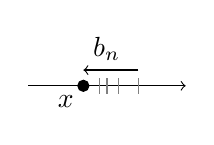
\begin{tikzpicture}[domain=-1:1.2]
	\draw[->](-0.7,0) -- (1.3, 0);
	\draw[->](0.7, 0.2) -- (0, 0.2)node[above right]{$b_n$};
 \draw[fill=black] (0,0) circle [radius=2pt] node[below left]{$x$};
	\foreach\i in {0.2, 0.45, 0.3, 0.7}
		\draw[ color=gray](\i,-0.1) -- (\i, 0.1);
    \end{tikzpicture}
}
    
    Но функция распределения \emph{непрерывна справа}.
    Значит, $$F_X(x) = F_Y(x) \qquad \forall x \in \mathbb{R}$$
\end{proof}
\end{theorem}
\begin{theorem} \label{lect12:th2}
    Если $\phi_X(\cdot) \in L^1(\mathbb{R})$, т.е. $\int_{\mathbb{R}} |\phi_X(t)| dt < \infty$, то случайная величина $X$ имеет непрерывную плотность, которая задается с помощью обратного преобразования Фурье:
    $$p(x) = \frac{1}{2\pi}\int_\mathbb{R} e^{-itx} \phi_x(t) dt,\quad x\in \mathbb{R} $$
\end{theorem}
\begin{proof}
    Заметим, что $p$ "--- непрерывная функция (это доказывается аналогично тому, как мы доказывали аналогичное утверждение для характеристической функции, когда вместо $\phi$ было $P$. Возьмем $a, b, \in C(F_X)$. 

    По теореме Фубини
    \begin{gather*}
        \int_a^b p(x)\: dx = \int_a^b \frac{1}{2\pi}\int_\mathbb{R} e^{-itx}\phi_X(t)\:dt\: dx = \frac{1}{2\pi}\int_\mathbb{R}\left(\phi_X(t) \int_a^b e^{-itx} dx\right)dt = \\
        =\frac{1}{2\pi} \int_\mathbb{R} \phi_X(t) \frac{e^{-iat} - e^{-ibt}}{it}\:dt = \frac{1}{2\pi}\lim_{c\to \infty} \int_{-c}^c \phi_X(t) \frac{e^{-iat} - e^{-ibt}}{it}\:dt = F_X(b) - F_X(a)
    \end{gather*}
    \emph{Пояснение.} 
\begin{gather*}
    \left|\phi_X(t) \frac{e^{-ita} - e^{-itb}}{it} \right| \leqslant \underbrace{|\phi_X(t)|}_{\leqslant 1} \left|\frac{e^{-ita} - e^{-itb}}{it}\right|\\
    \left|\frac{e^{ita} = e^{-itb}}{it}\right| = \left|\frac{e^{iat} (1 - e^{-ibt + iat})}{t}\right| = \frac{\left|e^{-it(b-a)} - 1\right|}{|t|}  \leqslant \frac{|t(b-a)|}{|t|} = |b-a|
\end{gather*}
Выше мы применили предыдущую лемму \ref{lect12:lem1}. Значит, функция интегрируема и применение теоремы Фубини законно.
Итак, мы доказали, что
\begin{multline}\forall a, b \in C(F_X): \quad \int_a^b p(x) dx = F_X(b) - F_X(a) \implies \\\implies\int_x^y p(s) ds = F_X(y) - F_X(x)\quad \forall x, y \in \R
\end{multline}

\begin{nb}
     $p(s) > 0$
     \begin{proof}
         Предположим, в некоторой точке $x_0$ $p(x_0) < 0$. Тогда в окрестности этой точки функция тоже будет строго меньше 0.

         Возьмем $x, y, \; x < y$ из этой окрестности
         $$\int_x^y p(s) ds) = F_X(y) -F_X(x) < 0$$
         Это невозможно, так как $x < y$, функция $F_X(t)$ не убывает.
     \end{proof}
 \end{nb}
Итак, по теореме о монотонной сходимости:
$$\int_\mathbb{R} p(s) ds = 1$$
Введем меру $Q(B)=\int_Bp(s) \:dx,$ где $B$ "--- борелевское. Тем самым $Q$ "--- вероятность. Значит
$$Q = P_X \mbox{ на } \{(a, b], -\infty < a \leqslant b < \infty\} $$
Но множество полуинтервалов"--- $\pi$-система $\implies Q = P_X$ на $\mathcal{B}(\mathbb{R})$
\end{proof}
\begin{nb}
    Это формула, в отличие от общей, действует \textbf{\emph{не всегда}}, так как функция может быть и не интегрируема.
\end{nb}
Если $d > 1$, $(a, b] = (a_1, b_1]\times\ldots\times(a_d, b_d]$. Исключим из $\R^d$ вдоль каждой оси не более чем счетное множество точек таких, что $P_X$ от каждой гиперплоскости равно 0. Пусть $D$ полученное множество точек для которых мера положительна. Тогда также получим
$$P_X((a, b] ) = \lim_{c\to \infty} \frac{1}{(2\pi)^d}\int\limits_{[-c, c]} \prod_{k=1}^{d} \frac{e^{it_ka_k} - e^{-it_kb_k}}{it_k} \phi_X(t) \:dt$$
Аналогично теореме \ref{lect12:th2}:

Если $\phi_X(t) \in L^1(\mathbb{R}^d)$, то $\exists$ непрерывная плотность
$$p(x) = \frac{1}{(2\pi)^d}\int_{\mathbb{R}^d} e^{-i(tx)}\phi_X(t)dt, \quad x\in \mathbb{R}^d $$
\begin{theorem} \label{lect12:th3}
    Для случайного вектора $X = (X_1, \ldots, X_d)$ формула
    $$\phi_X(t) = \prod_{x=1}^d \phi_{X_k} (t_k)$$
    справедлива $\forall t = (t_1, \ldots, t_d) \in \R^d$ в том и только том случае, 

    когда $X_1, \ldots, X_d$ "--- независимые величины.
\begin{proof}
    \textbf{($\implies$)} Пусть $z_1, \ldots, z_d$ "--- независимые комплекснозначные величины, т.е. $z_k = u_k + iv_k,\quad k = 1,\ldots,d\:$, и независимы $(u_1, v_1),\ldots,(u_d, v_d)$

    Если $z_1, \ldots, z_d$ независимы и $z_k \in L^1(\Omega), \:k = 1,\ldots, d$, то
    $$\mathbb{E}(z_1, \ldots z_d) = \mathbb{E}((u_1 + iv_1)\cdot \ldots \cdot (u_d + iv_d)) = \mathbb{E}z_1 \cdot \ldots \cdot \mathbb{E}z_d$$
    Если раскрыть скобки в произведении, то получатся слагаемые вида $w_1 \cdot \ldots \cdot w_d$, где $w_k = (u_k$ либо $iv_k)$. По лемме о группировке
    \begin{gather*}
        \mathbb{E} (w_1\cdot \ldots \cdot w_d) = \mathbb{E} w_1 \cdot \ldots \cdot \mathbb{E}w_d \qquad \mathbb{E} (v_1\cdot \ldots \cdot v_d) = \mathbb{E} v_1 \cdot \ldots \cdot \mathbb{E}v_d \implies\\
        \implies(\mathbb{E}u_1 + i\mathbb{E}v_1) \ldots (\mathbb{E}u_d + i\mathbb{E}v_d)
    \end{gather*}
    Независимость $x_1, \ldots, x_d$ влечет независимость величин $$\cos{t_1x_1} + i\sin{t_1x_1}, \:\ldots,\:\cos{t_dx_d} + i\sin{t_dx_d}$$
    Тогда $\phi_x(t) = \mathbb{E} e^{i(t,x)} = \mathbb{E}\left( \prod\limits_{k=1}^d e^{it_kx_k}\right) = \prod\limits_{k=1}^d \mathbb{E} e^{it_kx_k} = \prod\limits_{k=1}^d \phi_{x_k}(t_k)$

    \textbf{($\impliedby$)} Возьмем независимые $Y_1, \ldots, Y_d$ такие, что распределения совпадают: $$P_{Y_k} = P_{x_k}, \; k = 1, \ldots, d$$
    Это возможно по теореме Ламницкого-Улема. Тогда, так как распрделения совпадают:
    $$\phi_{Y}(t) = \prod\limits_{k=1}^d \phi_{Y_k}(t) = \prod\limits_{k=1}^d \phi_{x_k}(t) = \phi_x(t)$$
    По теореме единственности $$P_X = P_Y = P_{Y_1} \times \ldots\times P_{Y_d} = P_{X_1} \times \ldots \times P_{X_d} \implies x_1, \ldots x_d \mbox{ "--- независимы}$$
\end{proof}
\end{theorem}
\begin{lemma} \label{lect12:lem2}
    Пусть $x_1, \ldots, x_n$ "--- независимые случайные векторы со значениями в $\mathbb{R}^{m}$. Тогда
    $$\phi_{x_1 + \ldots + x_n} (t) = \prod_1^n \phi_{x_k}(t) , \quad t \in R^m$$
\end{lemma}
\begin{proof}
    Сами. Доказательство аналогично доказательству предыдущей теоремы \ref{lect12:th3}, экспонента распадается в произведение экспонент.
\end{proof}
\begin{nb}
    Обратное не верно.
\end{nb}
\subsection{Фундаментальная теорема Прохорова}
\begin{definition} \label{lect12:def2}
    Семейство вероятностных мер $\{Q_n, n \in T\}$ заданных на метрическом пространстве $(S, \mathcal{B}(S))$ называется \emph{слабо относительно компактным}, если из любой последовательности $(Q_n)_{n\in\N}$ можно извлечь слабо сходящуюся подпоследовательность $(Q_n')_{n'\in\N}$ к некоторой мере $Q$.
\end{definition}
\begin{nb}
    Эта мера $Q$ автоматически вероятностная, но не обязана входить в рассматриваемое семейство.
\end{nb}
\begin{definition} \label{lect12:def3}
    Вероятностные меры $Q_n$ \emph{сходятся слабо} к $Q$ ($Q_n \Rightarrow Q$) на метрическом пространстве $(S, \mathcal{B}(S))$, если
    $\forall f\colon S\to\R, \; f\in \mathcal{B}(S) | \mathcal{B}(\R)$, непрерывной и ограниченной:
    $$\int_A f\: dQ_n \to \int_S f\:dQ$$
\end{definition}
\begin{definition} \label{lect12:def4}
    Семейство вероятностных мер $\{Q_n, n \in T\}$ называется \emph{плотными}, если 
    $$\forall \epsilon > 0 \; \exists \mbox{ компакт }K_\epsilon \subset S\colon Q_k(K_\epsilon) > 1- \epsilon \quad \forall u \in T$$
\end{definition}
\begin{theorem}[Прохоров] \label{lect12:th4}
    Плотное семейство вероятностных мер является слабо отностительно компактным. Если пространство $S$ польское (полное, сепарабельное), то любое слабо отностительно компактное семейство вероятностных мер является плотным.

    Таким образом, на польском пространстве семейство вероятностных мер плотно тогда и только тогда, когда оно слабо относительно компактно.
\end{theorem}
\subsection{Критерий слабой сходимости вероятностных мер}
    \begin{lemma} \label{lect12:lem3}
        Пусть $(Q_n)_{n \in \mathbb{N}}$ "--- плотное семейство вероятностных мер. Если \textbf{каждая} слабо сходящаяся подпоследовательность $(Q_{n'})$ сходится к одному и тому же пределу $Q$, то и $Q_n \Rightarrow Q, \; n \to \infty$.
    \end{lemma}
    \begin{proof}
        Предположим, что $Q_n \not \Rightarrow Q$. Тогда $\exists$ непрерывная и ограниченная $f\colon S\to \mathbb{R}$ такая, что
        $$\int_S f \:dQ_n \not \to \int_S f \: dQ$$
        Тогда существует $\epsilon > $ и подпоследовательность $(n')$ такие, что
        $$\left| \int_S f\:dQ_n - \int_S f\: dQ\right| > \epsilon$$
        По теореме Прохорова \ref{lect12:th4} находим подпоследовательность $(n'') \subset (n')$, что
        $$Q_{n''} \Rightarrow \widetilde{Q}$$
        По условию, $\widetilde{Q} = Q$. Следовательно,
        $$\left|\int_S f(x) \:Q_{n''}(dx) - \int_S f(x)\:Q(dx) \right|\to 0$$
        Приходим к противоречию.
    \end{proof}
    \begin{lemma} \label{lect12:lem4}
        Пусть $(Q_n)$ "--- плотное семейство мер на $\{\mathbb{R}^d, \mathcal{B}(\mathbb{R}^d)\}$ Тогда последовательность $(Q_n)$ имеет слабый предел в том и только том случае, когда
        $$\forall t \in \mathbb{R}^d \quad\exists \lim_{n \to \infty} \phi_n(t)$$
    \end{lemma}
    \begin{proof}
        Если $Q_n \Rightarrow Q$, то мы уже видели, что $\phi_n(t) \to \phi(t)\; \forall t \in \mathbb{R}^d$

        \textbf{Обратно}. Пусть $\phi_n(t) \to \phi(t) \quad \forall t \in \mathbb{R}^d, \; n \to \infty$.

        Поскольку семейство $Q_n$ плотно по условию, найдется подпоследовательность $(n')$ такая, что $Q_{n'} \Rightarrow Q$, где $Q$ некоторая вероятностная мера.

        Предположим, что $Q_n$ не имеет слабого предела. Тогда по лемме \ref{lect12:lem3} найдется подпоследовательность $(n'')\subset (n')$ такая, что $Q_{n''} \Rightarrow\widetilde Q,\quad \widetilde Q \ne Q$.

        Тогда по условию $\forall t\in \R^d\quad \exists \lim \phi_n(t)$, поэтому:
        \begin{gather*}
            \lim_{n' \to \infty} \int\limits_{\mathbb{R}^d} e^{i(t,x)} \:Q_{n'}(dx) = \lim_{n'' \to \infty} \int\limits_\mathbb{R} e^{i(t,x)} \:Q_{n''}(dx) \implies\\
            \implies \int_{\mathbb{R}^d} e^{i(t, x)}\: Q(dx) = \int_{\R^d} e^{i(t,x)}\: \widetilde Q(dx)
        \end{gather*}
        По теореме единственности \ref{lect12:th1}, получаем, что $Q = \widetilde Q$. Противоречие.
    \end{proof}

\boxed{\textbf{\emph{Дальнейшее было рассказано на консультации.}}}\\
\textbf{\emph{Не знаю, войдет ли всё в экзамен. Скорее всего "--- да.}}

    \begin{lemma} \label{lect12:lem5}
        Пусть $\phi$ "--- характеристическая функция меры $Q$ на $\{\mathbb{R}^d, \mathcal{B}(\mathbb{R}^d)\}$. Тогда $\forall a > 0$
        $$Q\left(\R^d \setminus \left[-\frac{2}{a}, \frac{2}{a}\right]^d\right) \leqslant \frac{2}{(2a)^d} \int\limits_{[-a, a]^d} (1 - Re(\phi(t)) \:dt$$
    \end{lemma}
    \begin{proof}
        Будем доказывать для $d = 1$.
        $$Re(\phi(t)) = \int\limits_\R \cos{tx}\:Q(dx)$$
        По теореме Фубини
        \begin{gather*}
            \frac{1}{2a} \int_{-a}^a (1 - Re\: \phi(t))\:dt = \frac{1}{2a} \int\limits_{[-a, a]} \int\limits_\R (1 - \cos{tx}) \:Q(dx) \:dt
            =\\= \int\limits_\R \frac{1}{2a} \int_{-a}^a (1 - \cos{tx})\: dt \:Q(dx)\\
            \int_{-a}^a \cos{tx} \:dt = \frac{\sin{tx}}{x} \biggm|_{-a}^a = \frac{2\sin{ax}}{x} \qquad (x \ne 0)
        \end{gather*}
        Теорему Фубини применять корректно, так как подынтегральная функция ограничена, а значит "--- интегрируема.

        Итак,
        \begin{multline*}
            \frac{1}{2a} \int_{-a}^a (1 - Re\:\phi(t))\: dt = \int\limits_\R \left(1 - \frac{\sin{ax}}{ax}\right) \:Q(dx) \geqslant\\\geqslant \!\!\!\!\int\limits_{\R \setminus \left[-\frac{2}{a}, \frac{2}{a}  \right]}\!\! \left(1 - \frac{\sin{ax}}{ax} \right)\:Q(dx) \geqslant \frac{1}{2} Q\left(\R\setminus\left[ -\frac{2}{a}, \frac{2}{a}\right]\right) 
        \end{multline*}
        Пояснение
        $$\left| \frac{\sin{u}}{u}\right| \leqslant \frac{1}{|u|} \leqslant \frac{1}{2}, \qquad |u| \geqslant2 $$
    \end{proof}
\begin{theorem}[непрерывность, Леви] \label{lect12:th5}
    Пусть $(Q_n)_{n \in \mathbb{N}}$ последовательность вероятностных мер на $(\mathbb{R}^d, \mathcal{B}(\mathbb{R}^d)), (\phi_n)_{n\in \mathbb{N}}$ последовательность характеристических функций этих мер. Тогда справедливы следующие утверждения:
    \begin{itemize}
        \item Если $Q_n \Rightarrow Q$, то $\phi_n(t) \to \phi(t), \;  n \to \infty \quad \forall t \in \R^d$, где $\phi$ "--- характеристическая функция $Q$
        \item Если $\phi_n(t) \to \phi(t) \quad \forall t \in \R^d, \; n \to \infty$  и $\phi$ непрерывна в точке $0\in\R^d$,\\то $\phi$ является характеристической функцией некоторой вероятностной меры $Q$ и $Q_n \Rightarrow Q, \; n \to \infty$.
    \end{itemize}
\end{theorem}
\begin{proof}
    Утверждение 1 \emph{очевидно}, так как
    $$\phi_n(t) = \int_{\mathbb{R}^d} e^{i(t, x)} \:Q_n(dx) \to \int_{\mathbb{R}^d} e^{(t, x)}\: Q(dx) = \phi(t)\qquad \forall t \in \R^d$$
    Для доказательства второго утверждения понадобятся 3 предыдущие леммы (леммы \ref{lect12:lem3}, \ref{lect12:lem4} и \ref{lect12:lem5}). 

    Все будем доказывать для случая $d=1$.
$$\phi_n(t)| \leqslant 1 \implies |\phi| \leqslant 1 $$
Заметим, что $\phi$ измеримо как предел измеримых функций. Значит, $\phi$ "--- интегрируема.
    $\phi$ непрерывно в точке $0$. Значит,
    $$\forall \epsilon > 0 \; \exists a = a(\epsilon)\colon 0 \leqslant 1 - Re\: \phi(t) \leqslant \frac{\epsilon}{4}$$
    \begin{nb}
        Комплекснозначная функция непрерывна тогда и только тогда, когда непрерывны её комплексная и вещественная часть.
    \end{nb}
    Заметим, что $\phi(0) = 1$, так как $\phi_n(0) = 1$.

    Тогда
    $$\frac{1}{a} \int_{-a}^a \underbrace{(1 - Re\:\phi(t))}_{\leqslant \frac{\epsilon}{4} }\:dt \leqslant \frac{\epsilon}{2} $$
    По теореме Лебега о мажорируемой сходимости
    $$\frac{1}{a} \int_{-a}^a (1 - Re\:\phi_n(t))\:dt \to \frac{1}{a} \int_{-a}^a (1 - Re\:\phi(t))\:dt$$
    Значит, $\forall n \geqslant N_0(\epsilon)$
    $$\frac{1}{a} \int_{-a}^a (1 - Re\:\phi_n(t))\:dt \leqslant \epsilon$$
    Тогда по лемме \ref{lect12:lem5}
    $$Q\left(\R\setminus \left[-\frac{2}{a}, \frac{2}{a}\right]\right) < \epsilon, \qquad n > N_0$$
Для любой вероятностной меры на $\{\mathbb{R}^d, \mathcal{B}(\mathbb{R}^d)\}$ верно
$$\forall \epsilon > 0 \; \exists b = b(\epsilon)\colon P(\R\setminus[-b, b] < \epsilon$$
Здесь мы воспользовались тем, что $[-b, b] \to \R$ и непрерывностью вероятностной меры.

У нас есть конечное число мер $Q_{n_1}, \ldots, Q_{N_0}$. Найдем $b_n = b_n(\epsilon)$ такое, что
$$Q_n(\R\setminus[-b_n, b_n]) < \epsilon, \qquad n = 1,\ldots,N_0$$
Возьмем
$$b_0 = \max{\left\{\frac{2}{a(\epsilon)}, b_1(\epsilon), \ldots, b_{N_0}(\epsilon) \right\}}$$
Тогда $\forall n \in \N\quad Q_n(\R\setminus [-b_0, b_0]) < \epsilon$. Плотность семейства мер $Q_n$ установлена.

По лемме \ref{lect12:lem4} получаем, что существует слабый предел $Q_n$ "--- $Q$. Тогда
$$\psi(t) = \phi(t), \qquad t \in \R$$
где $\psi$ "--- характеристическая функция меры $Q$.
Следовательно, $\phi$ "--- характеристическая функция меры $Q$ и $Q_n \Rightarrow Q$
\end{proof}

\begin{col}
    Если $Q, \;Q_n$  "--- вероятностные меры, то
    $Q_n \Rightarrow Q$ тогда и только тогда, когда $\phi_n(t) \to \phi(t) \quad \forall t \in \R$
\end{col}
\begin{example}
    \emph{Условие непрерывности в теореме Леви существенно.}

Возьмем характеристические функции такого вида (см. рис.). Это будут\\характеристические функции, так как:

    \parbox[b][5cm][t]{0.65\textwidth}{
\begin{proof}
    Если бы $\phi_n$ \emph{была} характеристической функций, то она была бы интегрируема. А значит, существует плотность (и она задается преобразованием Фурье). Эта плотность неотрицательна и интеграл равен 1. Значит, это плотность и мы нашли распределение, которому отвечает $\phi_n$.
\end{proof}
Заметим, что $$\phi_n(t) \to \begin{cases}
    1, &\text{ if }t = 0\\
    0, &\text{ if }t \ne 0
\end{cases}$$
}
\hfill
\parbox[b][5cm][t]{0.3\textwidth}{
    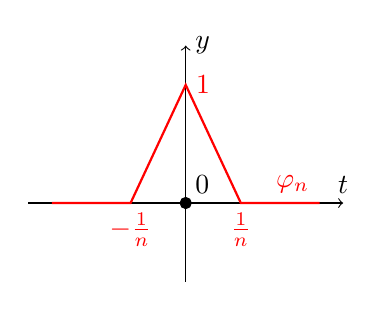
\begin{tikzpicture}
        \draw[->] (-2,0) -- (2,0) node[above]{$t$};
        \draw[->] (0, -1) -- (0, 2) node[right]{$y$};
        \draw[fill=black] (0,0) circle [radius=2pt] node[above right]{$0$};
		\draw[thick,color=red](-1.7,0)--(-0.7,0)node[below]{$-\frac{1}{n}$}--(0,1.5)node[right]{$1$}--(0.7,0)node[below]{$\frac{1}{n}$}--(1.7,0)node[above left]{$\varphi_n$};
    \end{tikzpicture}
}
Но предельная функция "--- не характеристическая, так как не непрерывна.
\end{example}
\end{document}
